\documentclass[letterpaper,12pt]{article}
\usepackage{fullpage}
\usepackage{fancyvrb,fancyhdr}
\usepackage{amsfonts}
\usepackage{array}
\usepackage{multirow}
\usepackage{amsmath, amssymb, amsthm}
\usepackage{graphicx,longtable, booktabs}
\usepackage[flushleft]{threeparttable}
\usepackage[footnotesize,center]{subfigure}
\usepackage{enumerate}
\usepackage{lastpage}
\usepackage{url}
\usepackage{mathrsfs}
\usepackage{cancel}
\usepackage{cite}
\usepackage{soul}
\usepackage{MnSymbol}
% Pseudo Code
\usepackage{algorithm}
\usepackage{algorithmic}
% Comments are in red
\usepackage{color}

\oddsidemargin 0in \evensidemargin 0in
\topmargin -0.5in \headheight 0.25in \headsep 0.25in
\textwidth 6.5in \textheight 9in %\marginparsep 0pt \marginparwidth 0pt
\parskip 0ex \parindent 10pt \footskip 20pt

\newfont{\bssten}{cmssbx10}
\newfont{\bssnine}{cmssbx10 scaled 900}
\newfont{\bssdoz}{cmssbx10 scaled 1200}

\pagestyle{fancy}
\fancyhead[LO]{\bssnine ConvNN used in DR classification }
% \fancyhead[R]{} \fancyhead[LO]{}
\fancyhead[RO]{\bssnine \thepage/\pageref{LastPage}}
%\fancyhead[RO]{\thepage}
\lfoot{} \cfoot{} \rfoot{}

%\usepackage[pdftex]{hyperref}

\def\t#1{{\tt #1}}
\newfont{\sserifn}{cmssbx10 at 11pt}
\newfont{\sserifo}{cmssbx10 at 12pt}

% Defining new \vect{} command to use a bold letter as a vector
\newcommand{\vect}[1]{\mathbf{#1}}
\newcommand{\erfc}{\mathrm{erfc}}
\newcommand{\figref}[1]{Figure~\ref{#1}}
\newcommand{\tableref}[1]{Table~\ref{#1}}
\newcommand{\eqsref}[1]{Eq.~\ref{#1}}
\newcommand{\algref}[1]{Algorithm~\ref{#1}}

%opening                    

\usepackage[para,multiple]{footmisc}
\newcommand{\jose}[1]{\comment{red}{#1}}
\newcommand{\imagej}{ImageJ }

\title{Convolution Neural Network Approach to Diagnosing Diabetic Retinopathy}
\author{Jos\'e Solomon \thanks{jose.e.solomon@gmail.com} } 

\date{}
\begin{document}

\maketitle
\begin{abstract}
This document discusses the fundamental concepts and results of my project on diabetic retinopathy diagnosis using convolution neural networks (ConvNN). It is derived from the Kaggle Diabetic Retinopathy Challenge \cite{kaggle} aimed at creating a robust algorithm to automate the process of classifying the level of diabetic retinopathy found in retinal scans. The fundamental components of ConvNN are introduced and the details of how these networks were trained are reviewed.
\end{abstract}
\tableofcontents

\section{Introduction}

There are two key facets to the project: first is the concept of the diabetic retinopathy and its diagnosis; the second is ConvNNs and their general functioning principles as applied to digital imaging processing and categorization. We begin with a cursory description of the former, and then focus the bulk of the theoretical discussion on the latter.

\section{Diabetic Retinopathy}

Diabetic retinopathy (DR) is a disease that generally afflicts those who have dealt with diabetes for a period of 5 years or more \cite{nih}. It is defined specifically as the deterioration of blood vessels found or that lead to the retina of the human eye, as illustrated in \figref{eye} below.

\begin{figure}[htbp]
\begin{center}
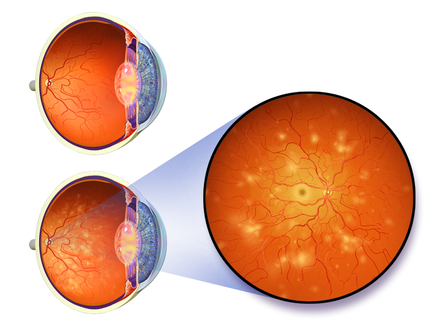
\includegraphics[scale=0.6]{images/illustration.png}
\caption{Diabetic retinopathy in comparison to a normal eye \cite{wiki}, (shown at the top left)}
\label{eye}
\end{center}
\end{figure}

The primary cause of DR is a byproduct of the condition of diabetes, where finer blood vessels in the human body tend to form abnormal branching structures and begin to exhibit thinning walls. This leads to deteriorated blood supply to the effected areas and eventually to hemorrhaging. In terms of the retina, this leads to blind spots forming in the person's field of vision. 

To diagnose the condition, a retinal scan of the eye is taken and a classification is assigned based on a combination of the following features: the number of abnormal vein branching seen, the general wall thickness of the blood vessels, and the number of blood stains observed due to hemorrhaging. DR is categorized on a scale from 0 to 4, and examples of level 0 and level 4 DR are shown in \figref{marking_image}. It should be noted that this method of categorizing DR is not fundamentally rigorous in nature and is more of a qualitative scale. 

\begin{figure}[htbp]
\begin{center}
 \subfigure[Level 0 DR]{\label{reference}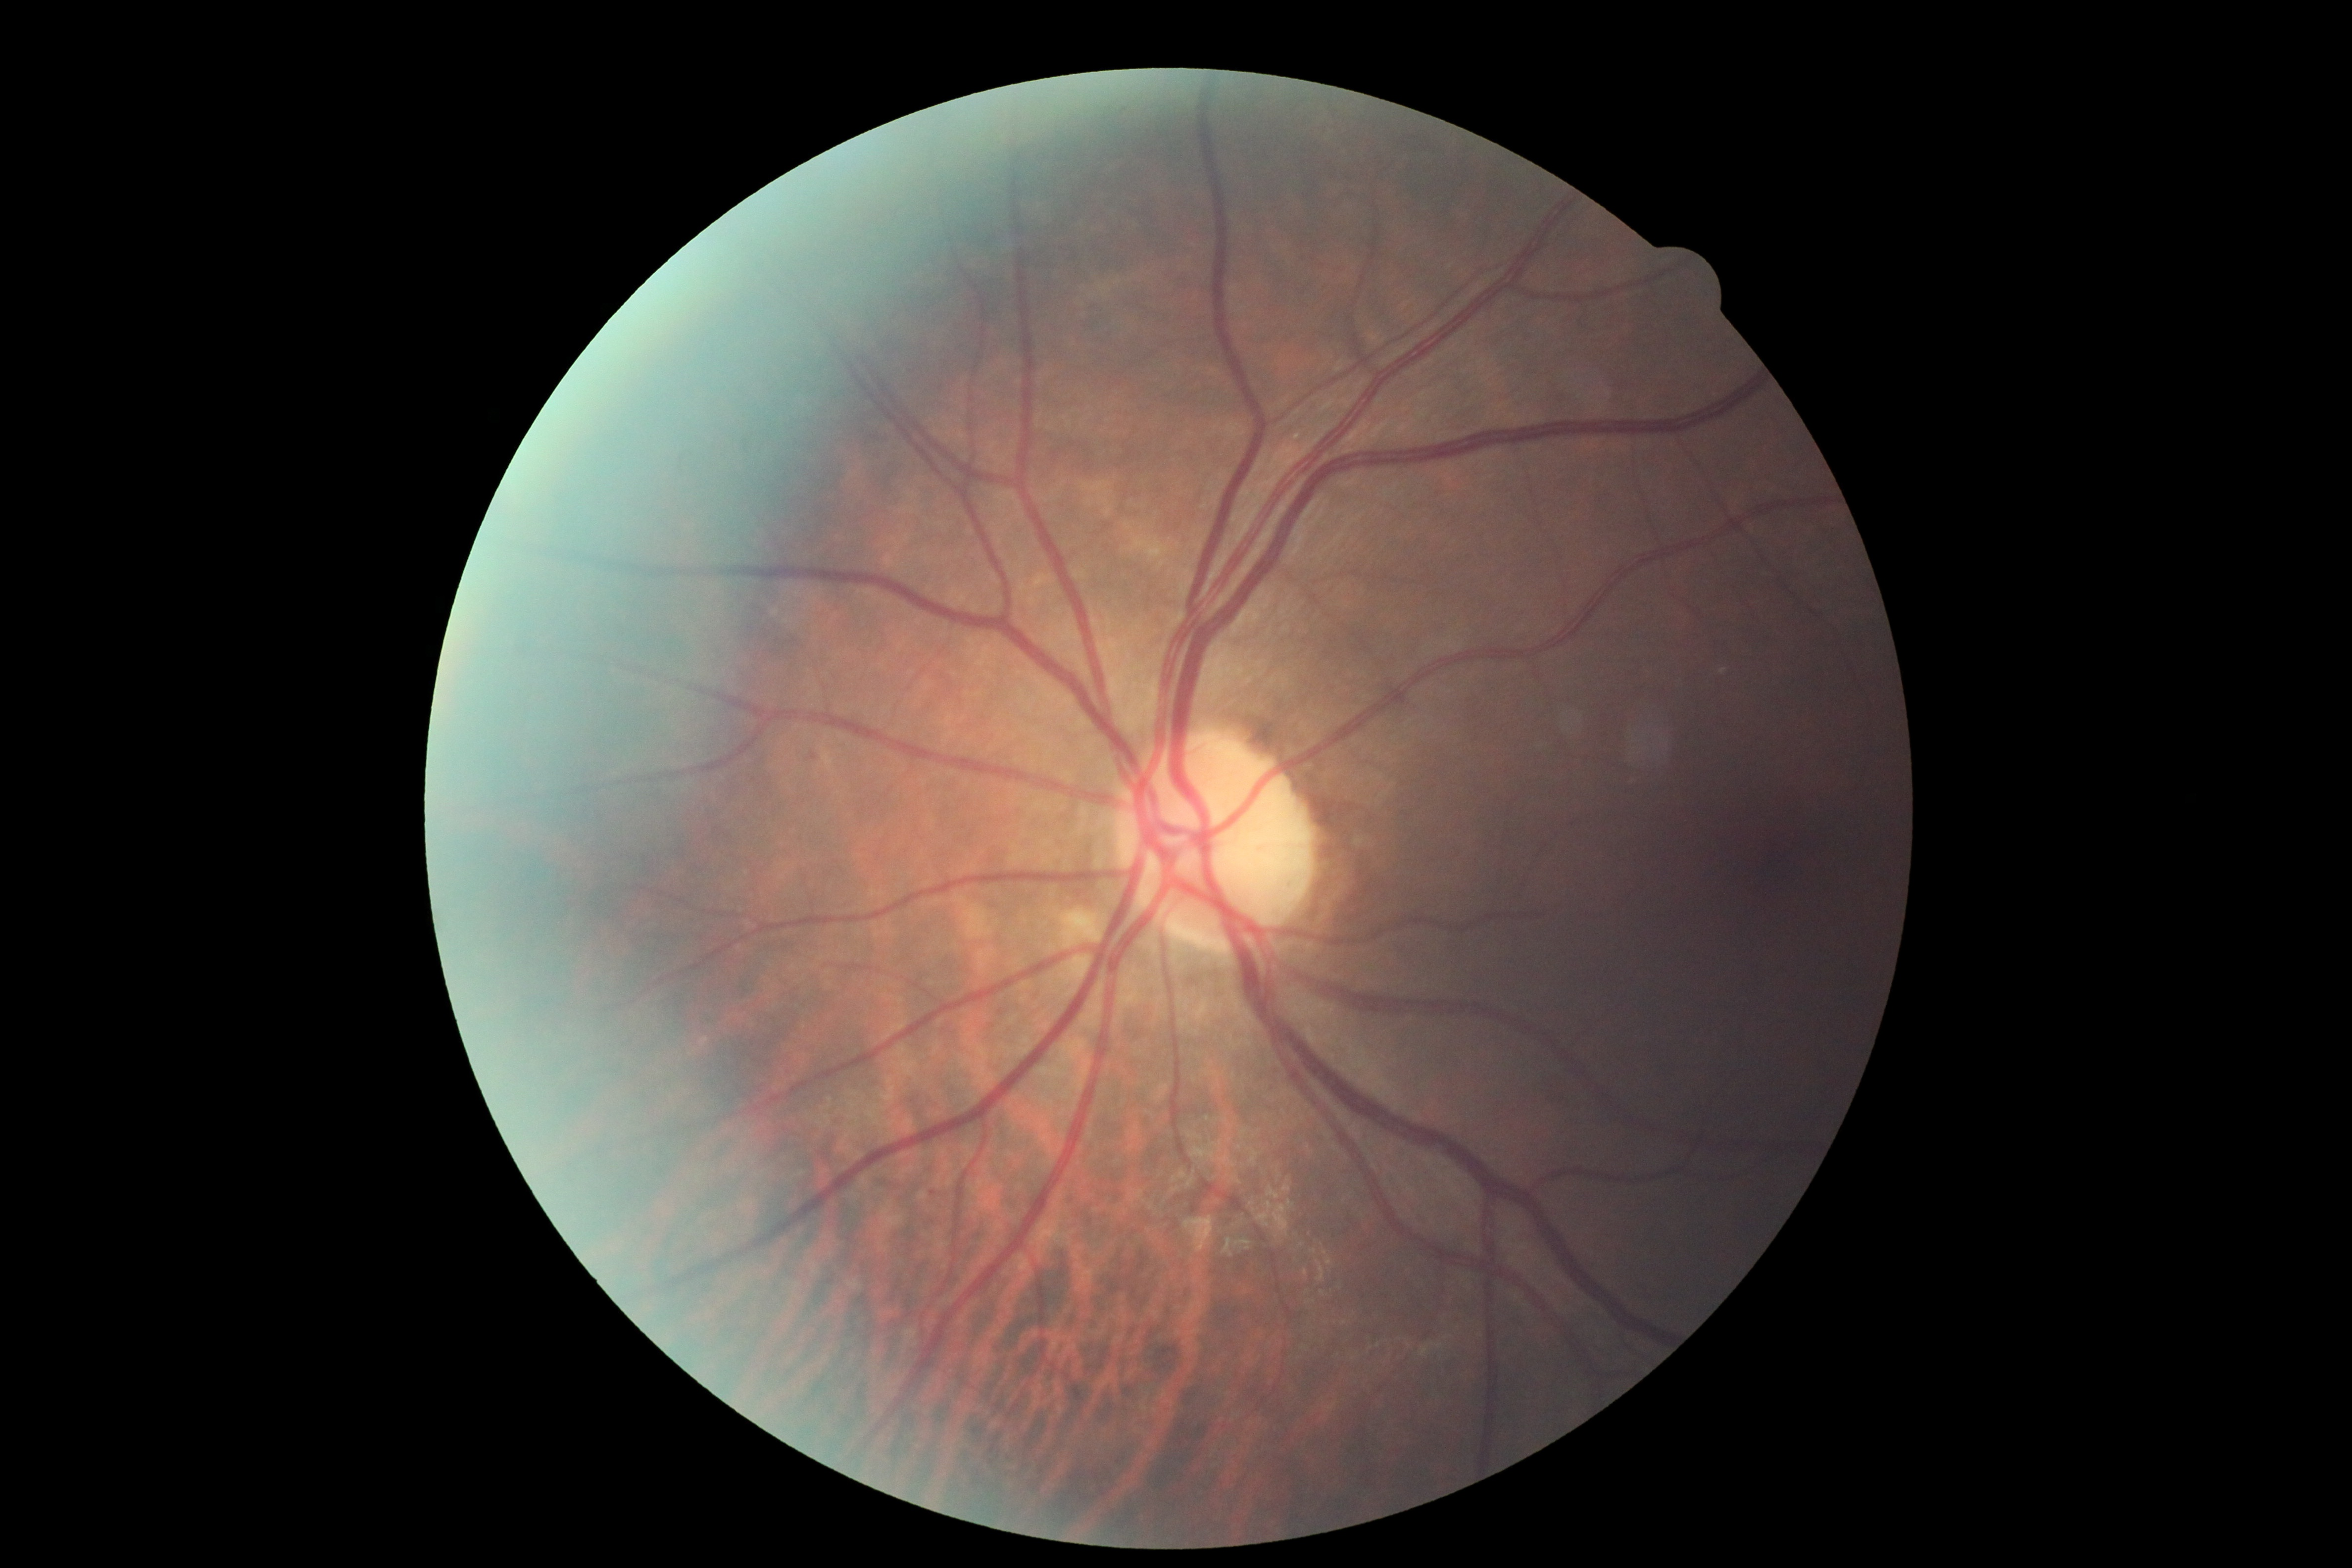
\includegraphics[scale=0.035]{images/0_Level_Example.jpeg}}
  \ \ \ \ 
\subfigure[Level 4 DR]{\label{new}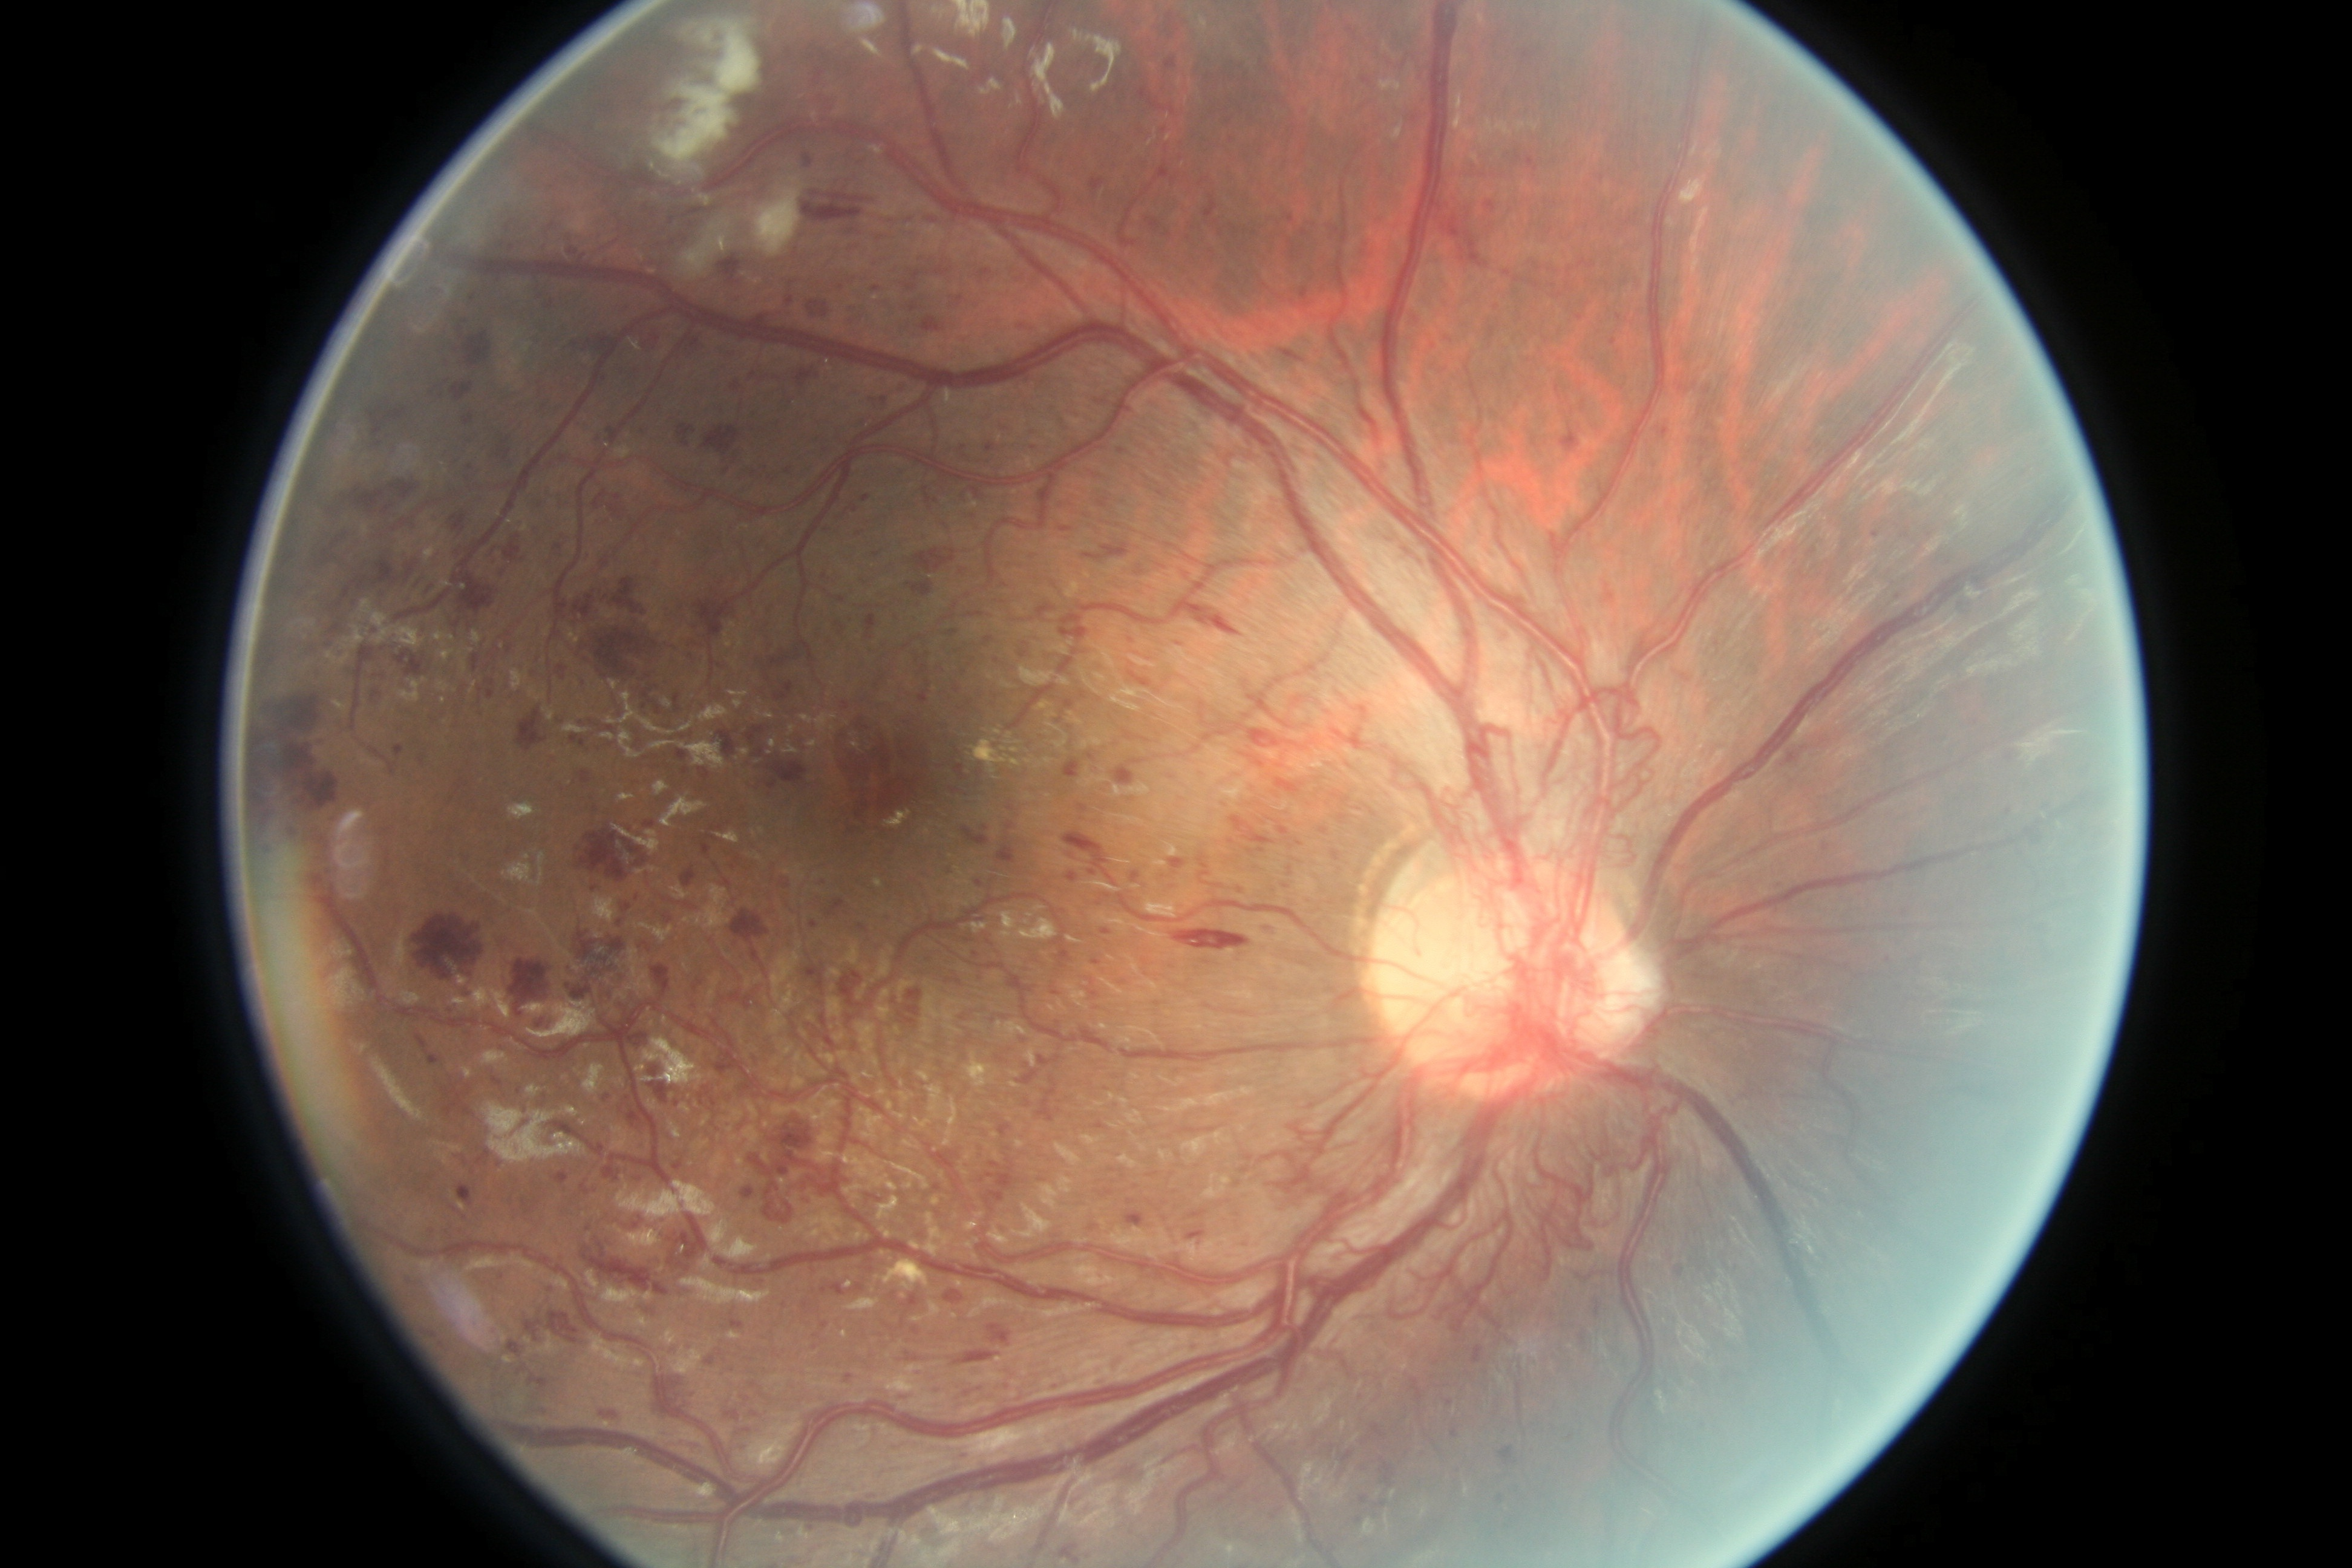
\includegraphics[scale=0.0425]{images/4_Level_Example.jpeg}}
\caption{Examples of level 0 and level 4 DR}
\label{marking_image}
\end{center}
\end{figure}

\subsection{The Kaggle Grand Challenge}

Kaggle has presented automated DR diagnosis as an open grand challenge. In doing so, Kaggle provided more than 35 gigabytes of retinal scan data, (over 35,000 images), where each image is roughly 1.5 megabytes in size. To aid in download and processing of the data set, Kaggle divided the image set into a training group and a testing group, and then subsequently divided each group into smaller subsets to facilitate file transfer. All the results presented here and in subsequent discussions are based on the first training set of images.

It is noted that the aim of the current work is to understand ConvNN from a fundamental perspective, and not to actually create a competitive solution for the grand challenge. Due to the size of the reference data set, and the limitations imposed by Python in terms of loading elements into shared memory, it would be very difficult to create a code base that could compete directly with other implementations in CuDa, (a GPU-level system language), which is the de facto favorite language for image processing.	

\section{Convolution Neural Networks}

ConvNN is a powerful machine learning technique that falls under the general premise of deep learning. There are number of flavors of ConvNN, but the specific implementation presented here is one derived from of the first concrete examples of the technique, the LeNet-5 \cite{LeNet}, which is especially adept at processing digital imaging.

The LeNet-5 consists of 3 primary component layers: the convolution layer, the pooling layer, and the conventional fully connected layer \cite{deep}. 

\subsection{The Convolution Layer}

The convolution layer is the work horse of the ConvNN, and it is what makes it such an indispensable tool for image processing. Mathematically, the concept of convolution is somewhat straightforward, and plays a key role in spectral methods/Fourier transform treatments. In terms of digital imaging, convolution can be expressed as \cite{deep} the product of the pixel intensity of a given image with that of a kernel, and is stated as
\begin{equation}
H[m,n] * G[m,n] \, = \, \sum_{u=- \infty}^{\infty} \sum_{u=- \infty}^{\infty} H[u,v] G[m-u, n-v]
\end{equation}

This may seem somewhat complex at first, but consider that a digital image is an array of pixels, each with an intensity that ranges from 0 up to a given bit depth, (e.g. 255 for 8-bit images). We can see that an image can be translated as matrix, where each element is a given pixel's image intensity. The concept is illustrated in \figref{lena}.
\begin{figure}[htbp]
\begin{center}
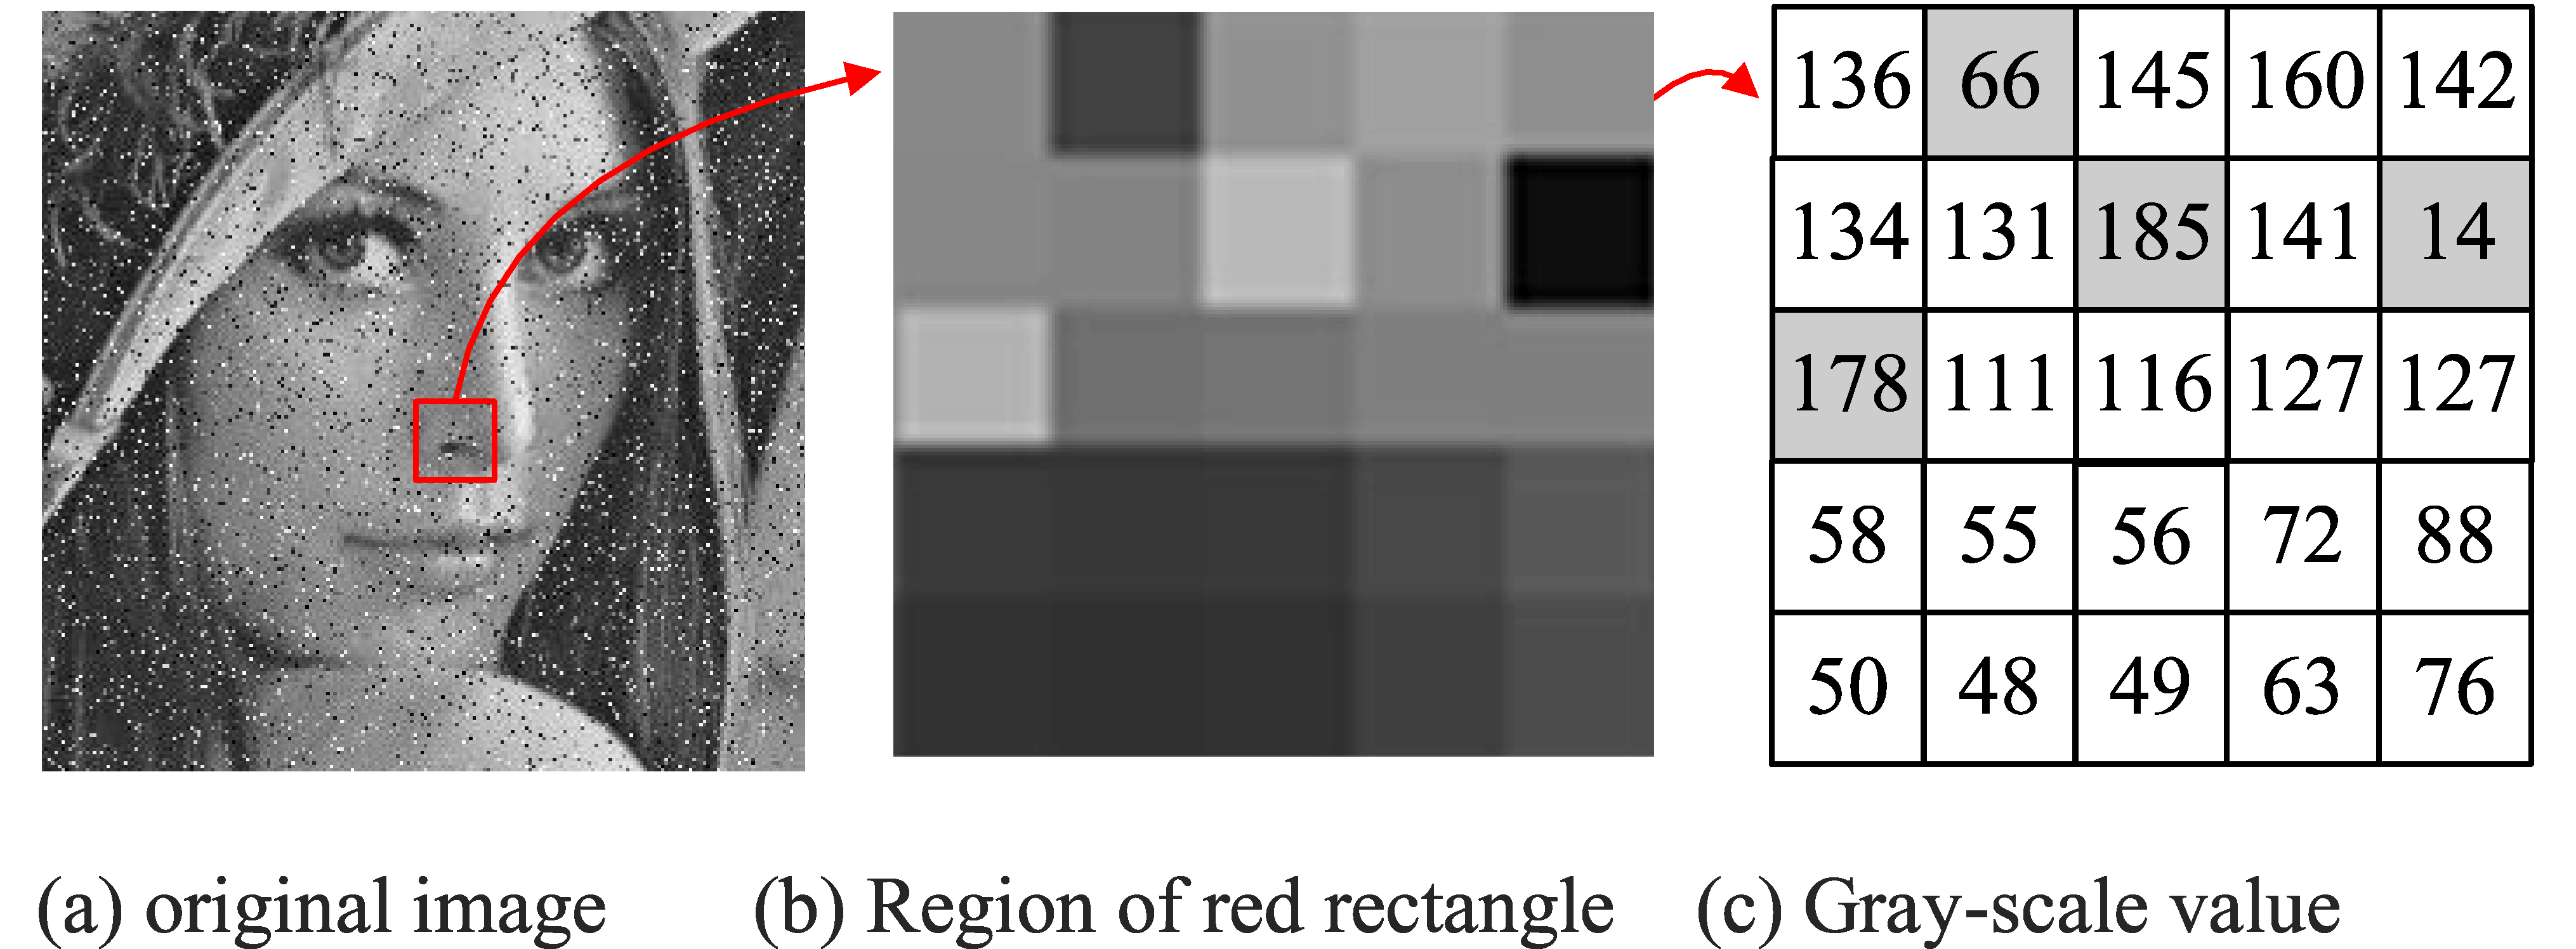
\includegraphics[scale=0.1]{images/lena.png}
\caption{Digital image as a matrix \cite{lena}}
\label{lena}
\end{center}
\end{figure}

With this concept in place, a kernel is itself a matrix of a prescribed dimension, smaller than that of the original image,  an example of which would be
\begin{equation}
H_{3 \times 3}^L \, = 
\begin{bmatrix}
  0 & 1  & 0 \\
  1 & -4 & 1 \\
  0 & 1  & 0
\end{bmatrix}
\label{lap_3x3}
\end{equation}

This matrix is applied, via convolution, across the matrix of the image to create a filtered image which, depending on the \textit{stride}, (i.e. number of times the kernel is applied across the original image), downsizes the original image into smaller matrix which is representative of the dot product between the original image and kernel.  The full convolution concept is illustrated in \figref{conv}. 

\begin{figure}[htbp]
\begin{center}
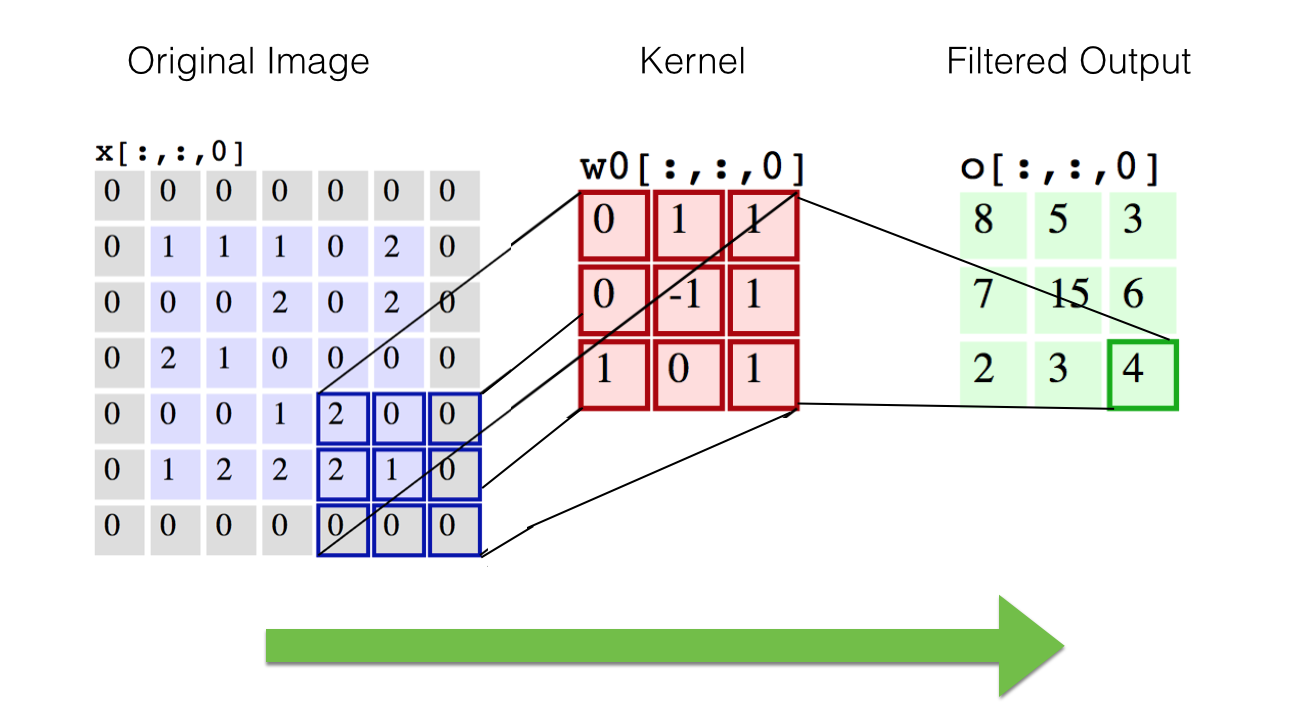
\includegraphics[scale=0.7]{images/convolution.png}
\caption{Convolution concept \cite{cs231}}
\label{conv}
\end{center}
\end{figure}

\subsection{The Pooling Layer}

In order to reduce the computational expenditure of the ConvNN algorithm, a pooling module is often used to reduce the required number of weights for a subsequent fully connected neural network layer.  

Usually the form of the pooling is \textit{max pooling}, where  a specific number of elements of the convoluted image are defined as common-pool members, (as illustrated in \figref{maxPool}), and only the pool member with the maximum value is carried forward in the network. The size of a pool is usually, but not required to be, the same size as the kernel applied during convolution. By focusing on the maximum value of a convolution, the network is becoming more sensitive to those image features which are more dominant in the total feature set.

\begin{figure}[htbp]
\begin{center}
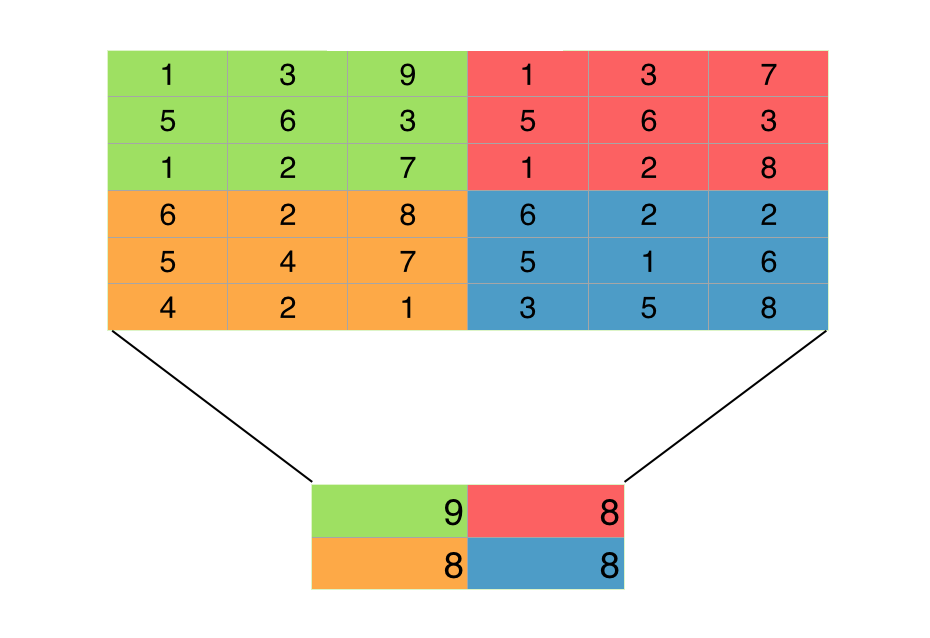
\includegraphics[scale=0.6]{images/maxpool.png}
\caption{Max pooling is where the largest value of each sub-cell is fed forward}
\label{maxPool}
\end{center}
\end{figure}

It is noted that a ConvNN often uses a series of convolution and pooling layers to continuously reduce the computational load of the final layer, or layers, of fully connected NN, which is normally the most computational expensive facet of the ConvNN pipeline. 

\subsection{The Fully Connected NN Layer}

The fully connected NN layer is actually a \textit{conventional} neural network, which is comprised of a series of nodes that are interconnected via a series of weights and bias units. Let's begin with the illustration shown in \figref{ann}.

\begin{figure}[htbp]
\begin{center}
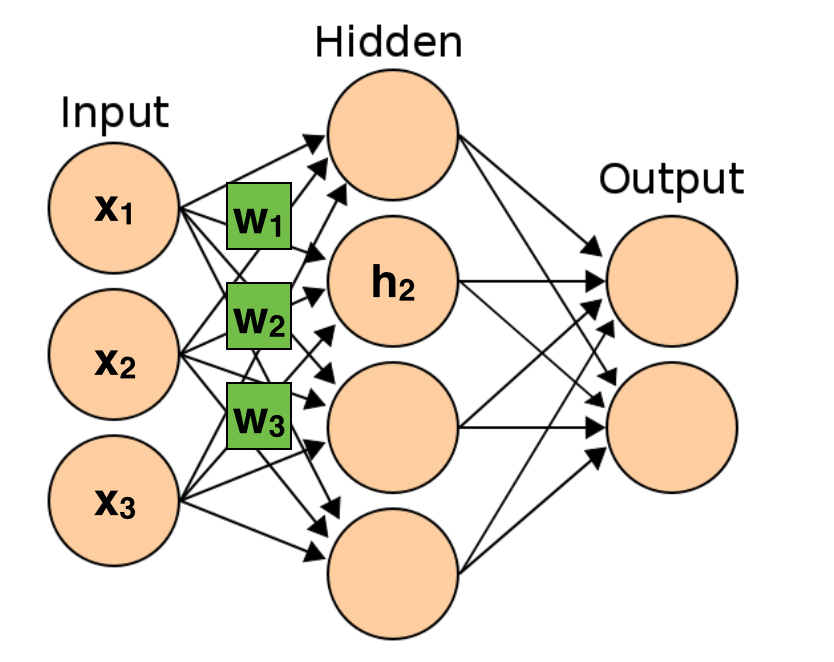
\includegraphics[scale=0.5]{images/nn_edit.png}
\caption{A fully connected neural network \cite{ann}}
\label{ann}
\end{center}
\end{figure}

As can be seen from the figure, each node is connected to the series of nodes in the layer directly downstream of it. The nodes downstream are in turn connected to each node in the layer directly upstream, as well as each node in the layer directly downstream. The result is a series of nodes that are \textit{fully} interconnected.

Let's say that for each input connection of a given node, there is an associated weight $w_i$. Given that there is $N$ number of nodes in the upstream layer, the input to the downstream node can be seen as 
\begin{equation}
f(\vec{w}^T\vec{x}) \, = f(w_0 \cdot x_0 + w_1 \cdot x_1 + \cdots + w_N \cdot x_N)
f_{reLu}(a) \, = \, \text{max}(0,a)
\end{equation}

We note that the dot product $\vec{w}^T\vec{x}$ is the input to a function, known as the activation function, which in turn is the input value of the downstream node. There are a variety of activation functions that can and have been used in NN. One of the most popular, and the one which is used here, is the \textit{tanh} activation function, which is defined as
\begin{equation}
f_{\text{tanh}}(a) \, = \frac{e^a-e^{-a}}{e^a+e^{-a}}
\end{equation}
which has an activation profile shown in \figref{tanh} As can be seen, the function has asymptotes  at 1 and -1 and exhibits positive values in $y$ for positive values of $x$. Another common activation function is the sigmoid activation function, which has a similar profile as \textit{tanh} and has the functional form
\begin{equation}
f_{sigmoid}(a) \, = \frac{1}{1-e^{-a}}
\end{equation}
As shown in \figref{sig}, the sigmoid activation function has asymptotes at 1 and 0, and is centered at the origin in $x$ and at 0.5 in $y$. 

Another popular variant, and the one that was ultimately used to provide the final set of results, is the rectifier activation function, (commonly referred to as a \textit{ReLu}), defined as
\begin{equation}
f_{ReLu}(x) \, = \, \text{max}(0,x)
\end{equation}
This is very straightforward activation function, illustrated in \figref{relu}, that tends to have more favorable characteristics from the perspective of backward propagation, which is the \textit{learning} process of the network.
\begin{figure}[htbp]
\begin{center}
 \subfigure[Tanh Function]{\label{tanh}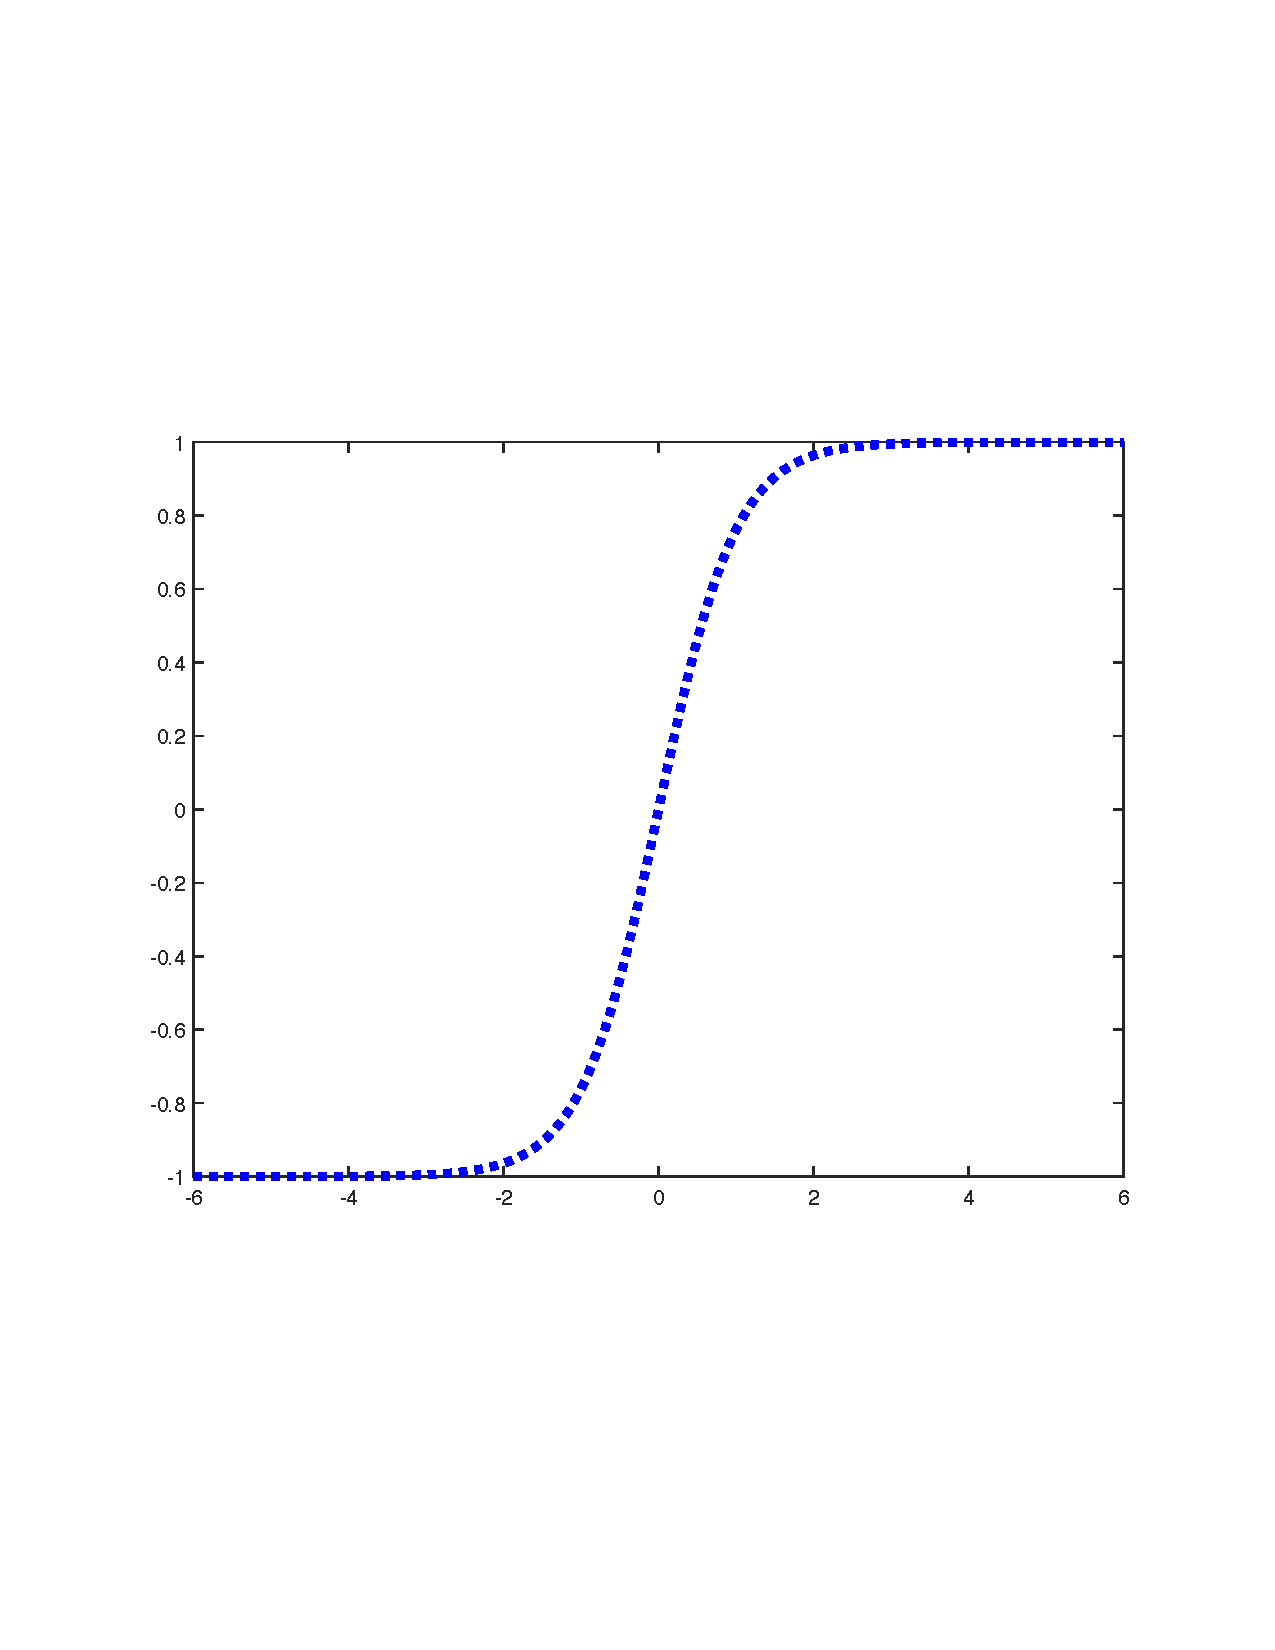
\includegraphics[scale=0.45]{images/TanhFunction.pdf}}
  \ \ \ \ 
\subfigure[Sigmoid Function]{\label{sig}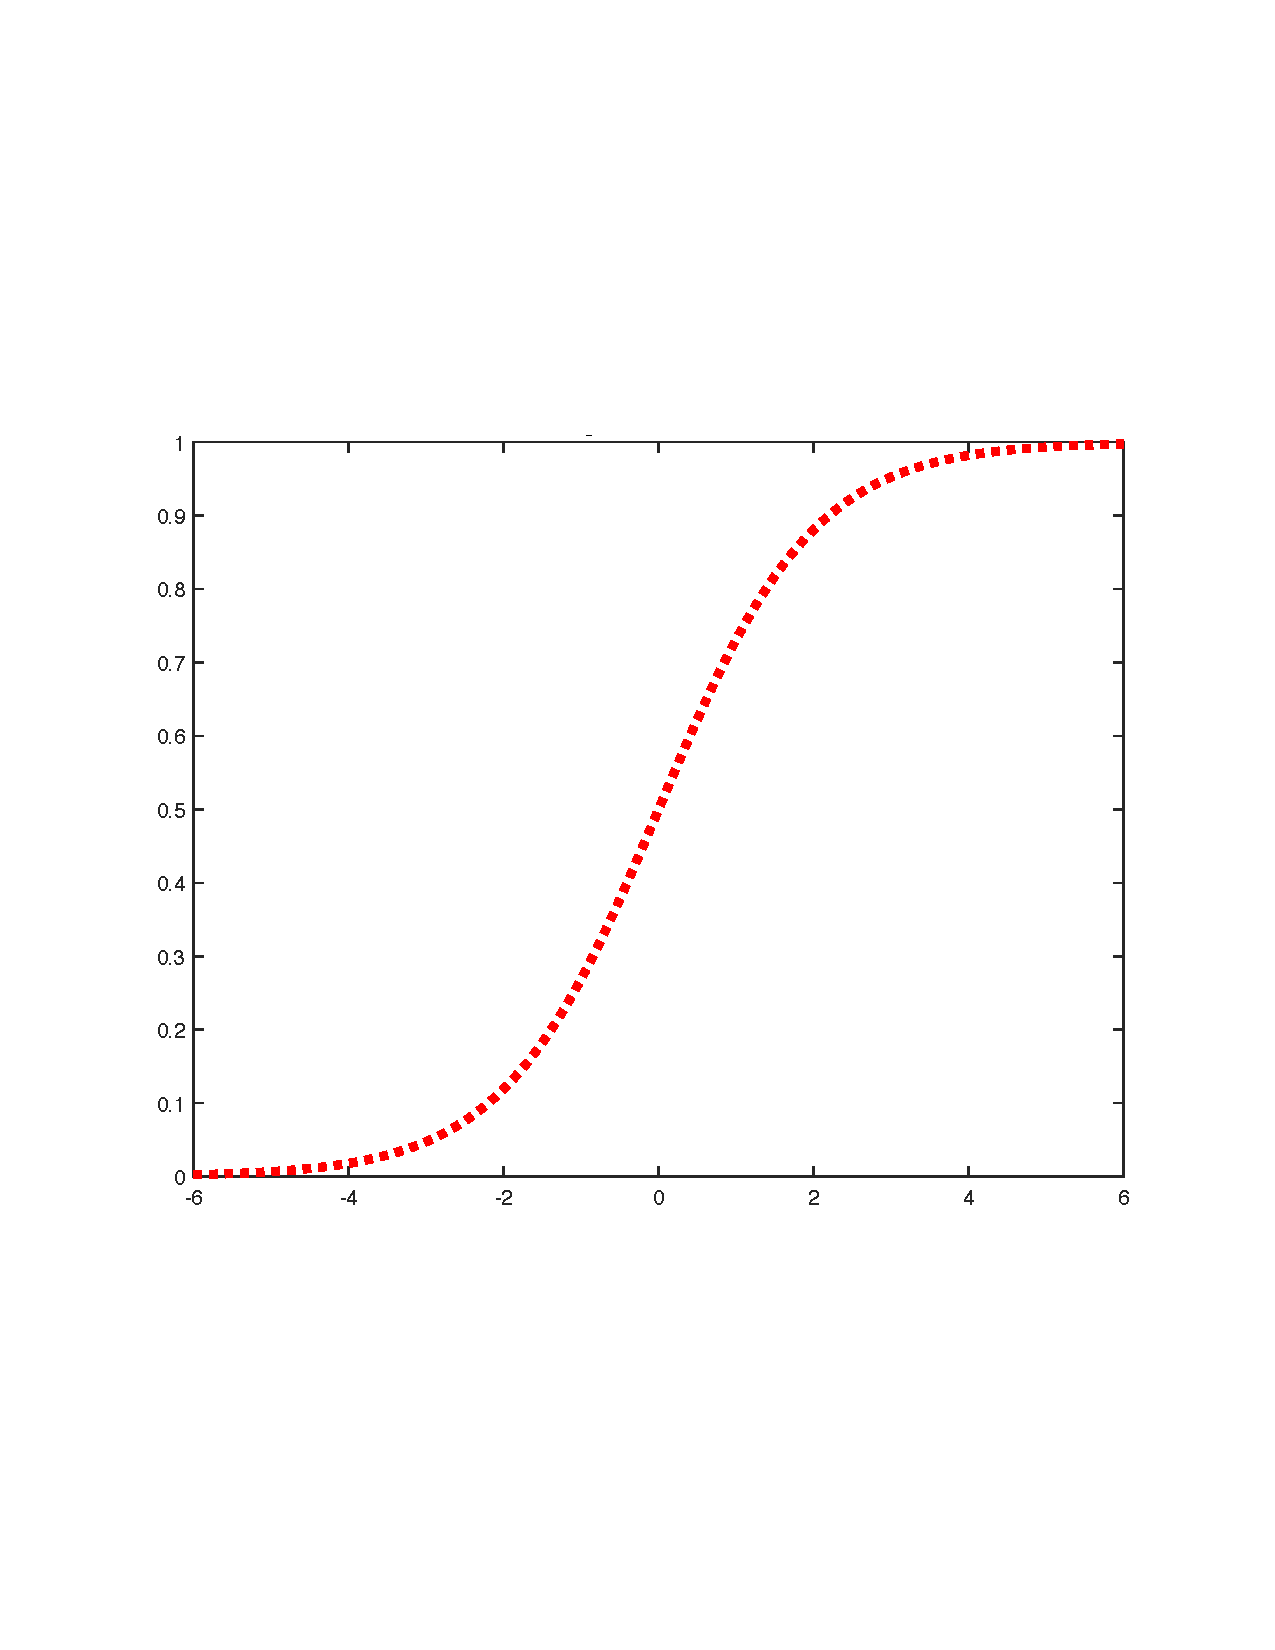
\includegraphics[scale=0.45]{images/SigFunction.pdf}}
  \ \ \ \ 
\subfigure[ReLu Function]{\label{relu}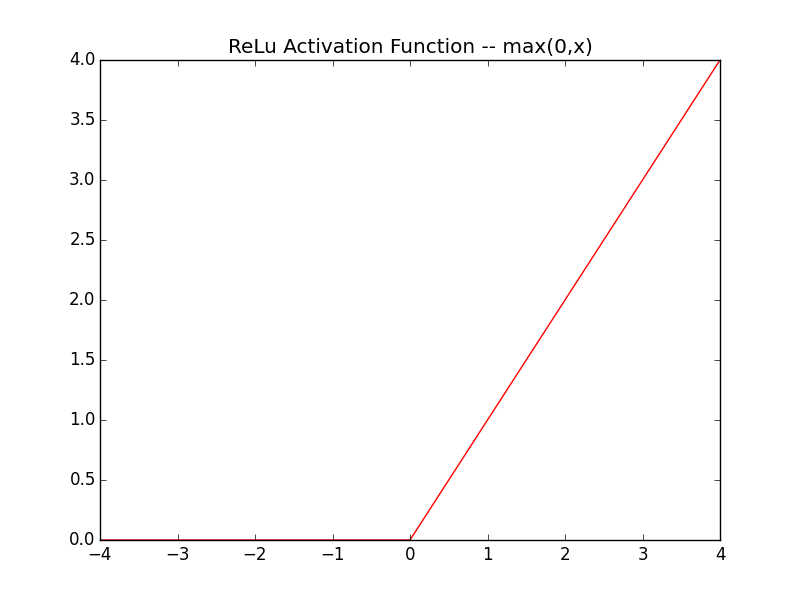
\includegraphics[scale=0.45]{images/reLu.png}}
\caption{NN activation functions}
\label{marking_image}
\end{center}
\end{figure}

The sigmoid and \textit{tanh} activation function are commonly used, but the \textit{ReLu} activation is gaining more traction in terms of ConvNN due to the favorable back-propagation properties, (i.e. the learning process of the NN). Back-propagation is a key concept in NN and ConvNN, but its description is beyond the scope of the current document.

\subsection{Logistic Regression Node}

The final layer of the ConvNN is usually a classifier. In the attempted implementation by the author, the logistic regression function was used as the output node. This is a classifier reviewed in class and it's functional form is \cite{deep} and sometimes labeled as a \textit{softmax} classifier.
\begin{equation}
y_{prediction} \, = \, \text{argmax} P_i (Y = i | \{x, w\})
\end{equation}
where the probability is
\begin{equation}
P_i \, = \, \frac{e^{\vec{w}_i^T \vec{x}_i}}{\sum_j \vec{w}_j^T \vec{x}_j }
\end{equation}
This simply means that the output of the NN is mapped to one of the label of classes, (in this case the level of DR which ranges from 0 to 4).

\subsection{Summary}

So putting all the pieces together,  the ConvNN has the general layout seen in \figref{summary}

\begin{figure}[htbp]
\begin{center}
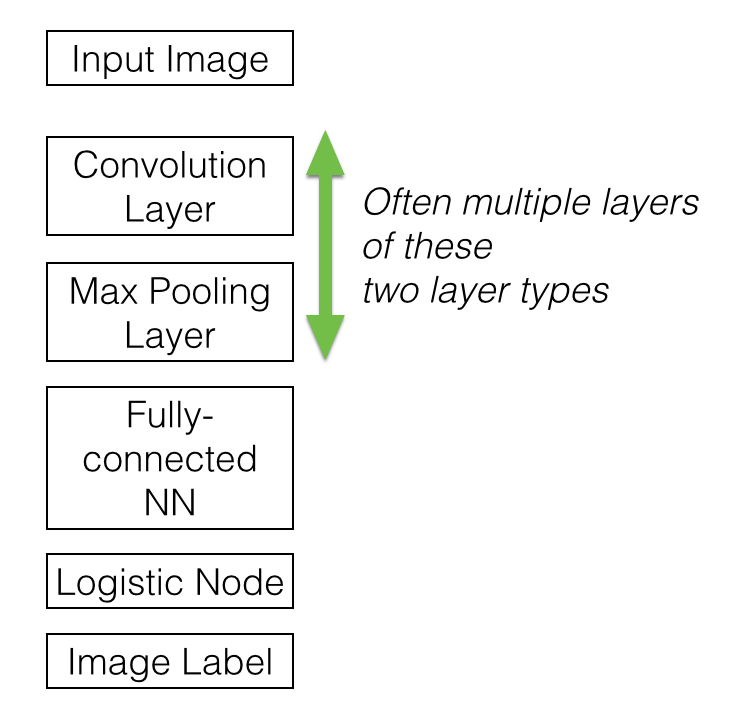
\includegraphics[scale=0.6]{images/summaryNN.png}
\caption{The ConvNN as a whole}
\label{summary}
\end{center}
\end{figure}

As noted in the figure, the convolution layer and the max pooling layer are often stacked multiple times in practice to reduce the overall computational load of the fully connected neural network module, which is often the most computational expensive member of the ConvNN. In the author's implementation, three convolution/pooling layers where stacked before output was connected to the fully-connected neural network. In the final functional network, which was implemented using NVIDIA's Digits \cite{digits}, seven convolution layers where used with pooling interspersed throughout the different junctures of the network.

\section{Actual Implementation}

Python is a powerful and flexible language, but it is not entirely ideal to deal with image processing. An initial attempt to code a ConvNN using the Theano library \cite{theano} was hampered by excessively long run times that prohibited debugging of the code base or real analysis of the results.

To manage the challenges of handling such large images in conjunction with the issues related to memory management of Python code, a move was made to run code using the Digits framework, which implements ConvNN within the framework of a Graphic Processing Unit, (GPU), architecture. GPUs have significant advantages over Central Processing Units, (CPUs), implementations when it comes to processing digital images for a number of reasons. Mainly, GPUs consist of a high number of cores who are optimized to segregate shared memory instances and run individual processes on subsets of the larger instance. This comes about from the GPU's  primary function: to take a large image, break it down into smaller subsections and send it to your display interface. By leveraging GPUs to break up an image matrix into smaller matrices, run convolution/pooling/fully-connected NN on the image sub-samples, and then tying things back together in the final classifier node, a GPU implementation can be order of magnitudes faster than standard, serial CPU implementation.

This section will discuss the architecture of the ConvNN that was used to produce most of the results documented, but first a concise review will be given on image pre-processing which was required before actual ConvNN training could begin.

\subsection{Image Preparation}

To process images, the \textit{openCV} computer vision library was initially used to load, crop and convert to gray-scale all images in the selected training set. Below is an excerpt from the code that does some of this processing. Once images are loaded and cropped they look as shown in \figref{loaded}.

\begin{verbatim}
 def processD(self):
        # Load left image
        for i in range(0,len(self.lImageNames)):
            print 'Left images being loaded: ' + str(i)
            name = self.imageDPath+self.lImageNames[i]+'.jpeg'
            image = cv2.imread(name,4)
            # crop the image
            image = image[10:2010,610:3010]
            # convert to gray scale
            imageL = cv2.cvtColor(image, cv2.COLOR_BGR2GRAY)
            self.lImageList.append(imageL)
\end{verbatim}

\begin{figure}[htbp]
\begin{center}
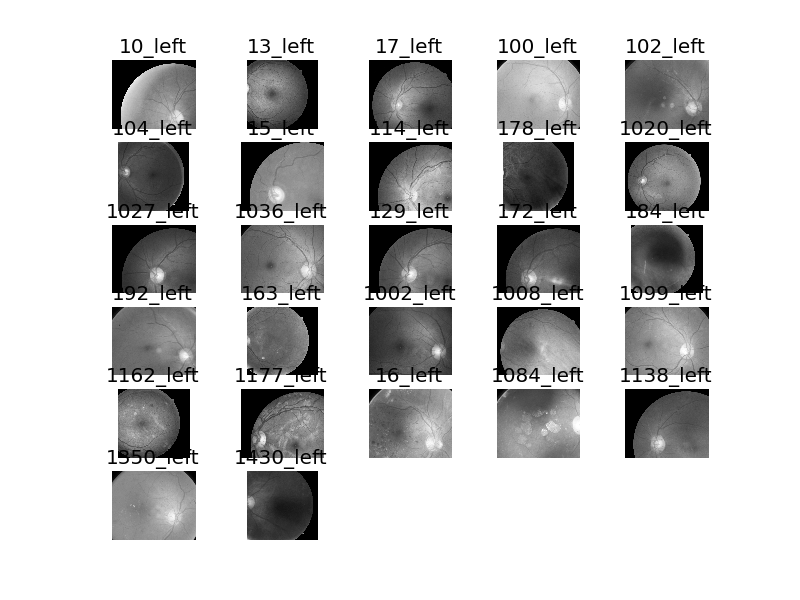
\includegraphics[scale=0.5]{images/lInitialImages_gray.png}
\caption{Images loaded, cropped, and converted to gray-scale}
\label{loaded}
\end{center}
\end{figure}

Initial testing found that color is actually a very significant aspect of the diagnosing procedure, and so a different method of cropping and reducing the size of image was used using the textit{imagemagik} toolbox. Resulting images where converted from \textit{jpeg} to \textit{png} file format and went from roughly 4000x2500 pixels to 256x256 pixels, resulting in image file size reductions from ~9 Mb to ~66 Kb. This conversion made image handling much more manageable for the ConvNN training. An example image is presented in \figref{png}.

\begin{figure}[htbp]
\begin{center}
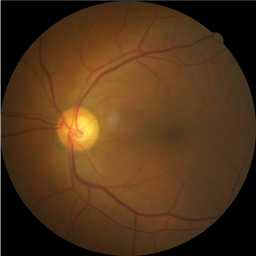
\includegraphics[scale=0.75]{images/png_format.png}
\caption{A down-sampled and cropped \textit{PNG} image} 
\label{png}
\end{center}
\end{figure}

In addition to considerations of the image file sizes, care had to be given as to the number of images given to the network representing each of the different levels of DR. \textit{Kaggle} has provided training images in five installments. Filtering through the labels for all training images, it is seen from \figref{fullSample} that most of the data is heavily skewed toward lower levels of DR, (level 2 and below). To create a more robust training set, equal number of samples of each DR level is being fed to the ConvNN. 

\begin{figure}[htbp]
\begin{center}
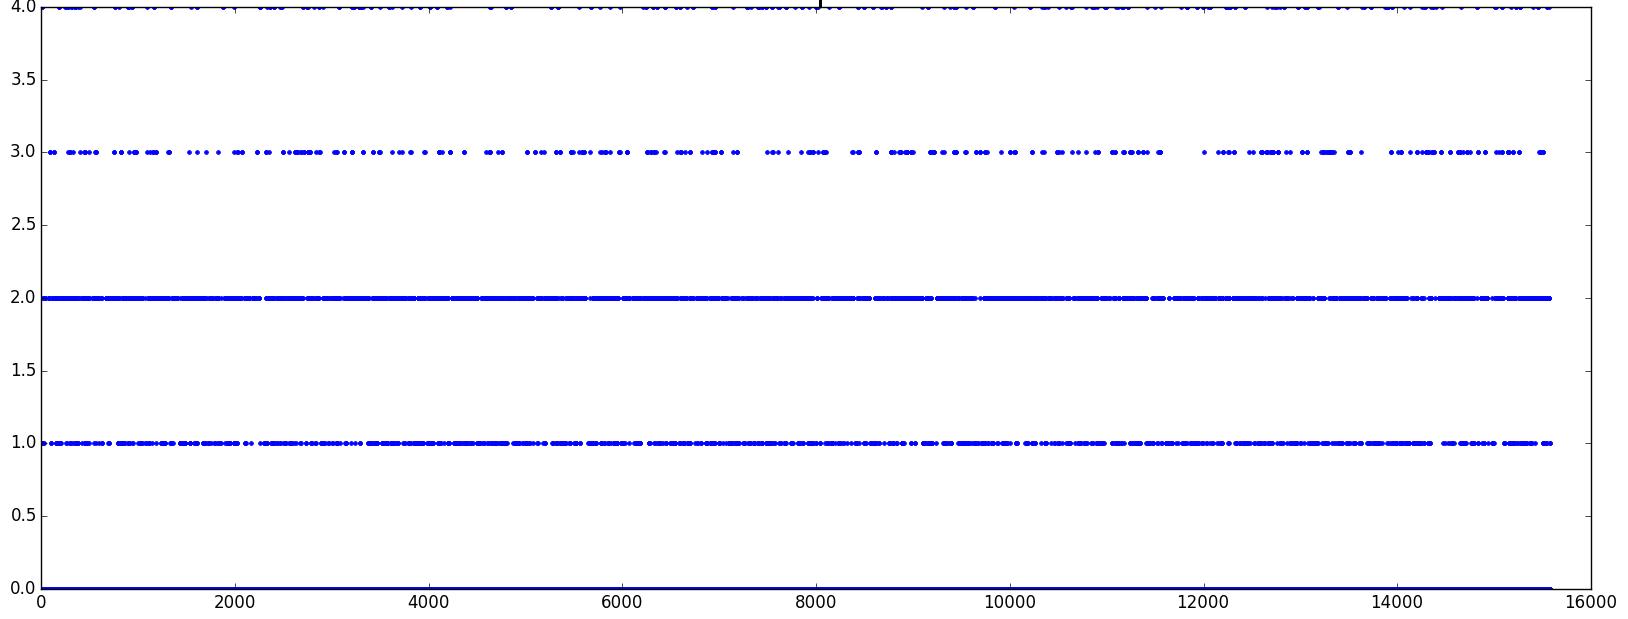
\includegraphics[scale=0.25]{images/FullSample.png}
\caption{All the labels of the training data}
\label{fullSample}
\end{center}
\end{figure}

A code was written to filter the images from the training set, giving the distribution show in \figref{filtered}.

\begin{figure}[htbp]
\begin{center}
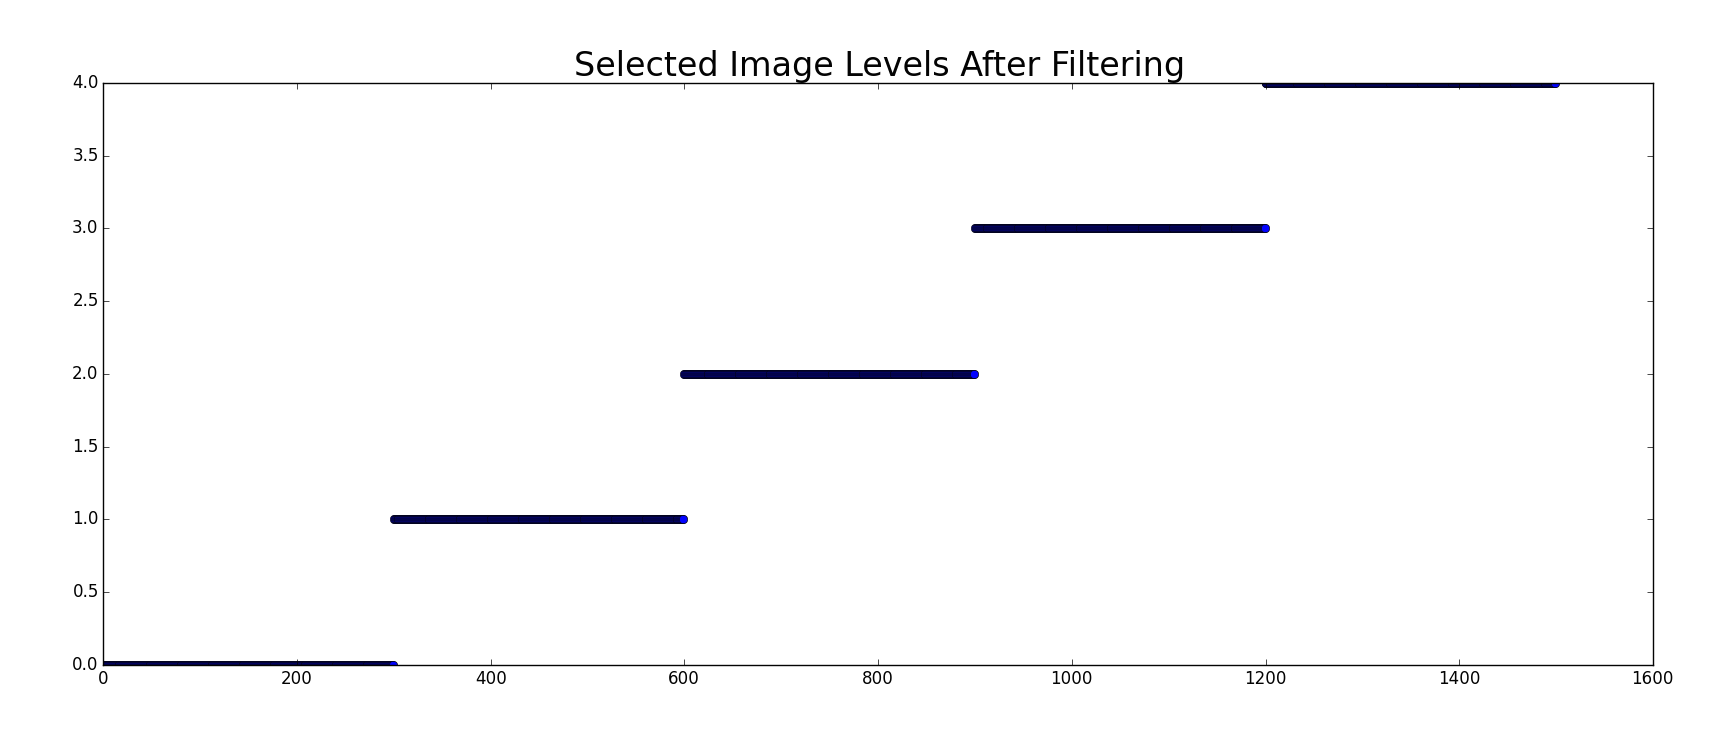
\includegraphics[scale=0.25]{images/After_filtering.png}
\caption{Equal number of DR samples for each category}
\label{filtered}
\end{center}
\end{figure}

\subsection{Customized \textit{AlexNet}}

Using \textit{Digits}, two popular ConvNN documeted in the literature were tested. These were the \textit{GoogLeNet} \cite{GoogLeNet} and the \textit{AlexNet} \cite{AlexNet}. By testing data sets with these base implementations, the author was able to fine tune the number of images given to the network to represent each level of DR. Using insight gained from these initial results, a customized \textit{AlexNet}was created that had a larger initial filter size for the starting convolution layers. The aim was to be able to capture with greater accuracy the characteristic blotches representative of blood hemorrhaging in the retina. The customized \textit{AlexNet} used for the final classification results shown in the next section is depicted in \figref{alexnet} below.

\begin{figure}[htbp]
\begin{center}
\subfigure{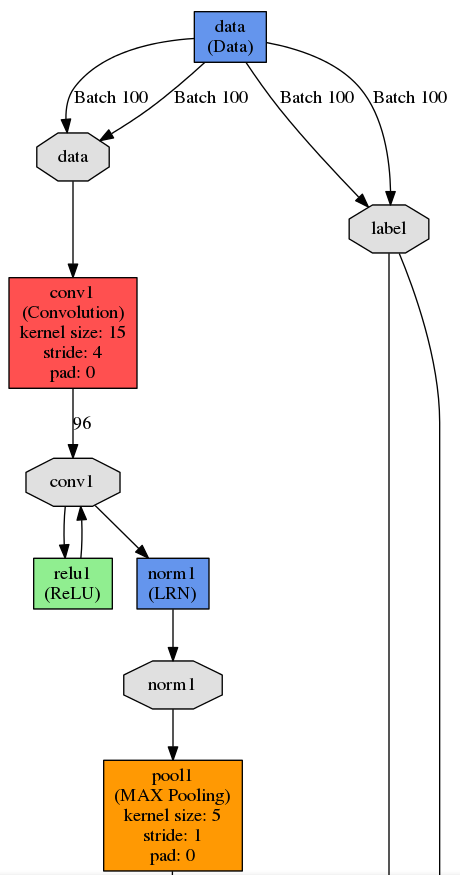
\includegraphics[scale=0.25]{images/Part1.png}}
\subfigure{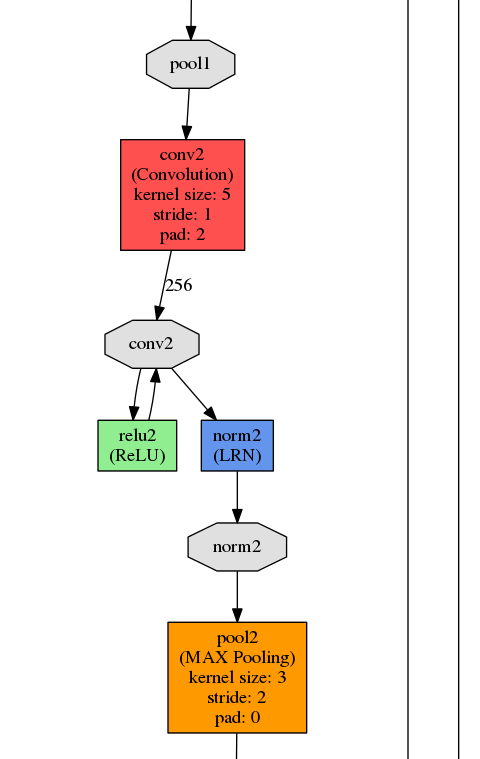
\includegraphics[scale=0.25]{images/Part2.png}}
\subfigure{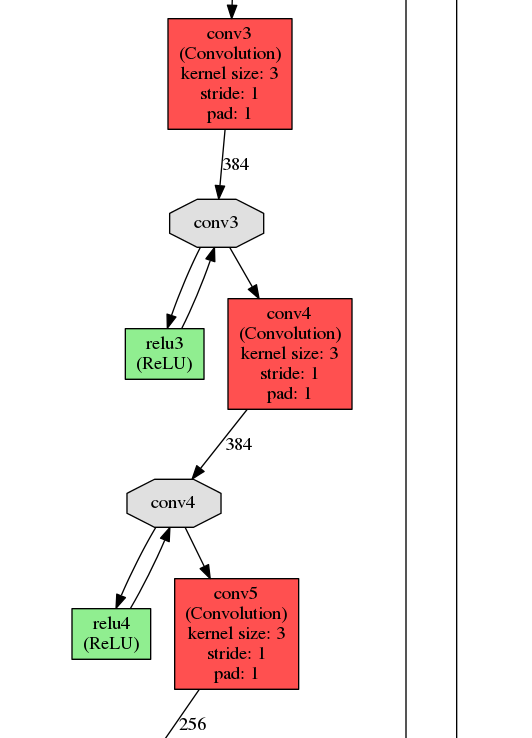
\includegraphics[scale=0.25]{images/Part3.png}}
\subfigure{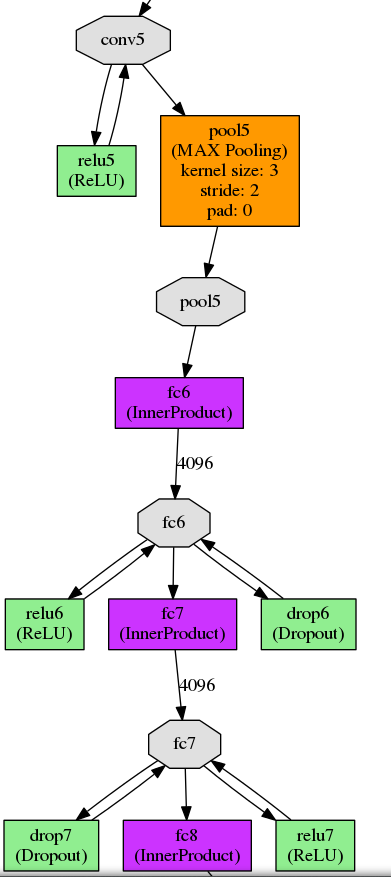
\includegraphics[scale=0.25]{images/Part4.png}}
\subfigure{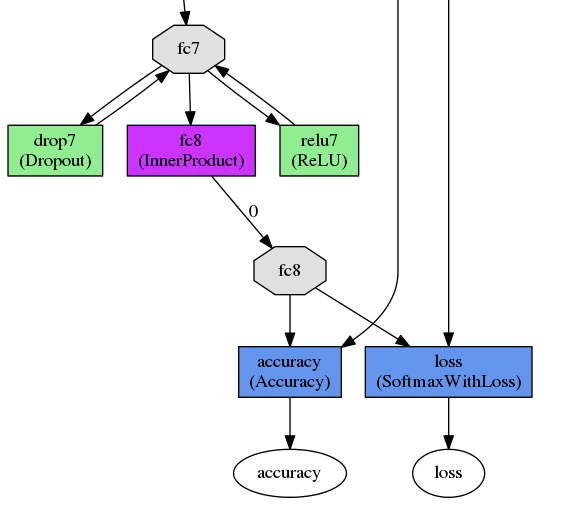
\includegraphics[scale=0.2]{images/Part5.png}}
\caption{Customized AlexNet with larger intake filter size and pooling layers, (illustration should be read from left to right, top to bottom at each column)}
\label{alexnet}
\end{center}
\end{figure}

\section{Results}

The results of the work will be presented in two parts: the first will be a series of binary-based results that help fine tuning the balance of images given to train the ConvNNs. The second set will be the final classification network that gave the best results overall. 

\subsection{Binary Classification Networks}

To gain a better understanding of the number of images required to perform a robust training of a ConvNN, (which was evident based on ad-hoc initial attempts of throwing images at the networks and seeing dismal results), a binary study was done in which retinal scans with no DR where compared with retinal scans exhibiting DR, and the network was expected to discern between the two. These results are presented here.

\subsubsection{DR 0 vs DR 4}

To start the study off, scans with no DR, (i.e. Level 0), where compared to those showing the maximum level of DR at Level 4. The normalized confusion matrix for a data set composed of 200 images for each of the DR levels using a \textit{GoogLenet} ConvNN is shown in \figref{DR0_DR4}. The accuracy of the classification was 53.38 $\%$.

\begin{figure}[htbp]
\begin{center}
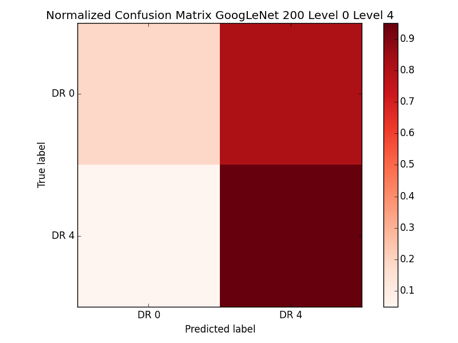
\includegraphics[scale=0.5]{images/Normalized_DR0_DR4.png}
\caption{DR 0 vs DR 4 Normalized Confusion Matrix}
\label{DR0_DR4}
\end{center}
\end{figure}

The minimum certainty of the network for each classification, shown in \figref{C_DR0_DR4}, shows a certain sparsity at the lower confidence regime for DR Level 4 classification. That indicates that the network is less confident when diagnosing Level 4 versus diagnosing Level 0, indicating that number of images used in this training set should be increased.

\begin{figure}[htbp]
\begin{center}
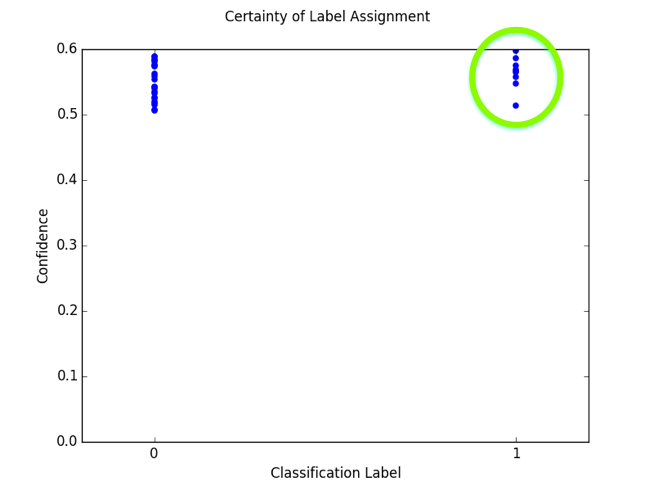
\includegraphics[scale=0.5]{images/Certainty_DR0_DR4.png}
\caption{DR 0 vs DR 4 Certainty Comparison}
\label{C_DR0_DR4}
\end{center}
\end{figure}

\subsubsection{DR 0 vs DR 3 \& DR 4}

Increasing the number of images to 400 for each level of DR to be classified, and adding DR Level 3 images to the mix, showed an improvement in the accuracy of the network. Using 400 images for each DR level, and combining together levels 3 and 4 to see if the network can use a more detailed feature space of the presence of DR, a \textit{GoogLeNet} was able to achieve 55.15 $\%$. The normalized confusion matrix and certainty plot are shown in \figref{DR0_DR3_4}.

\begin{figure}[htbp]
\begin{center}
\subfigure{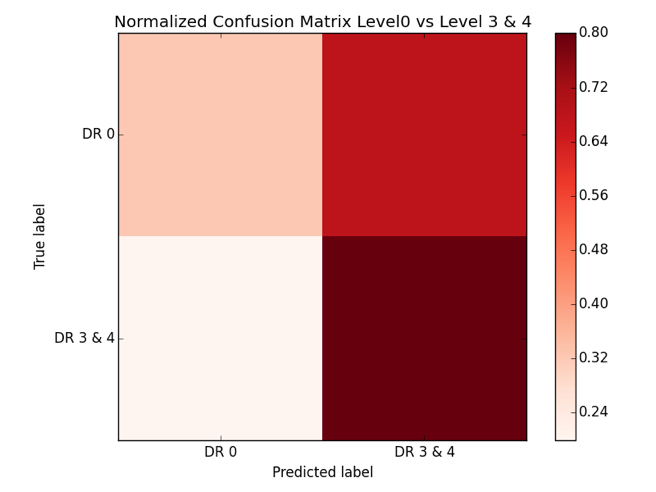
\includegraphics[scale=0.35]{images/Normalized_CM_DR0_DR3_4.png}}
\subfigure{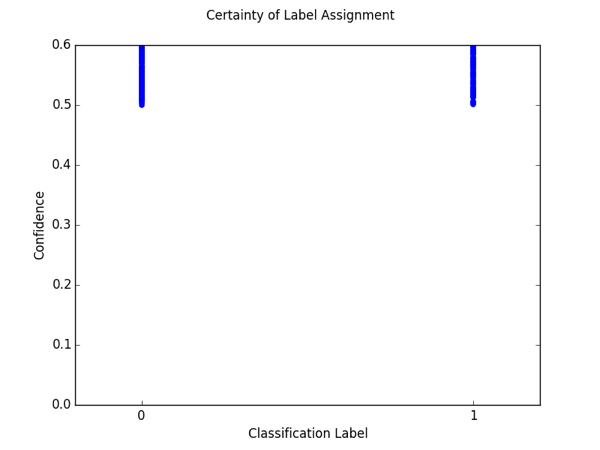
\includegraphics[scale=0.35]{images/C_DR0_DR3_4.png}}
\caption{Normalized Confusion Matrix and Certainty Distribution for DR 0 vs DR 3 \& 4 Training Set)}
\label{DR0_DR3_4}
\end{center}
\end{figure}

The results indicate some improvement in the certainty distribution of the network, showing less sparsity in the minimum confidence required to issue a classification. The next step was to add an even greater number of images to each level of DR.

\subsubsection{DR 0 vs DR 1-4}

Using 1000 images for Level DR 0 and roughly 600 images per level of DR for Levels 1 through 4, a binary training was done using a \textit{GoogLeNet} once again. The results are shown in \figref{DR0_DR+}. The overall accuracy for the network was 58.70 $\%$.

\begin{figure}[htbp]
\begin{center}
\subfigure{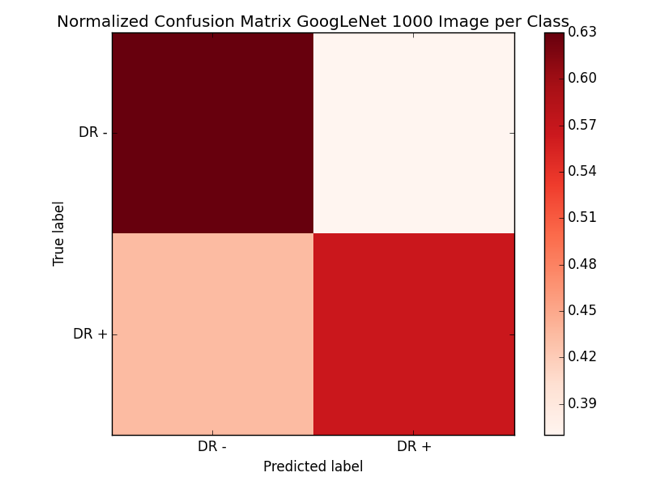
\includegraphics[scale=0.35]{images/Normalized_CM_DR0_DR+.png}}
\subfigure{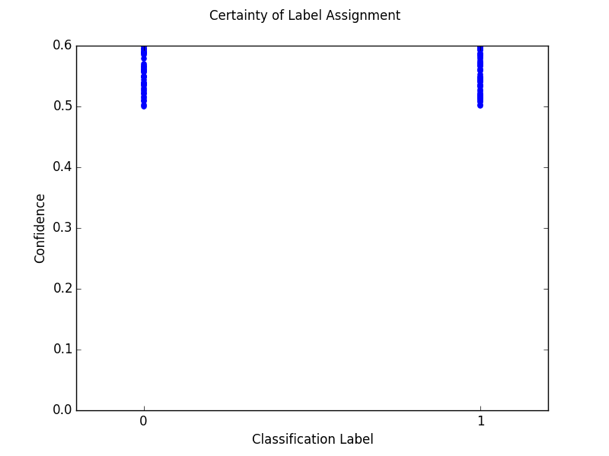
\includegraphics[scale=0.35]{images/C_DR0_DR+.png}}
\caption{Normalized Confusion Matrix and Certainty Distribution for DR 0 vs DR 1-4)}
\label{DR0_DR+}
\end{center}
\end{figure}

The results indicate a uniform certainty for each classification, (no DR versus some level of DR), so a move was made to due actual diagnosing of DR level, which is done next.

\subsection{Category Classification Network}

Studying the results of the binary classification, a customized \textit{AlexNet} was created as discussed in the previous section and illustrated in \figref{alexnet}. The primary modification to the base \textit{AlexNet} given in \cite{AlexNet} was to increase the size of the first layer convolution's kernel so as to try to capture with greater fidelity some of the blood blotches so frequently seen in DR retinal scans. Using this customized network, the normalized confusion matrix and certainty distribution shown in \figref{DR0_C} were achieved. The overall accuracy of the trained network was 39.32 $\%$.

\begin{figure}[htbp]
\begin{center}
\subfigure{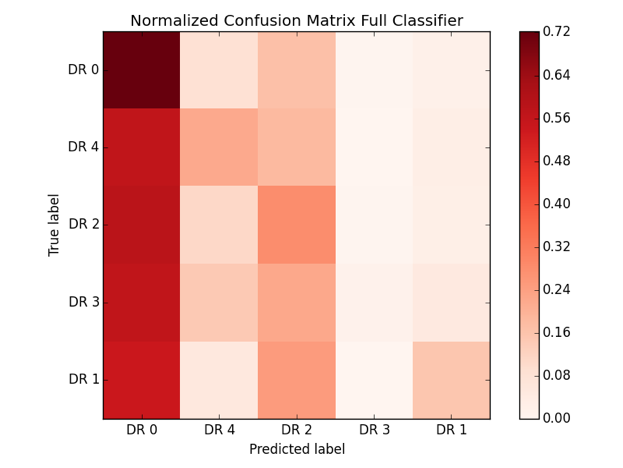
\includegraphics[scale=0.35]{images/Normalized_CM.png}}
\subfigure{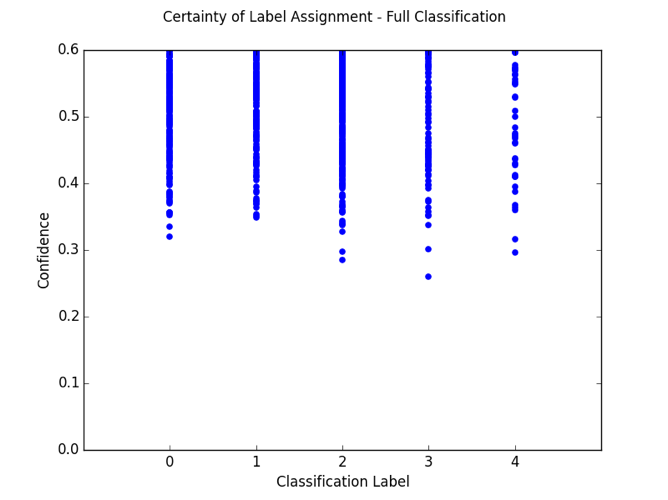
\includegraphics[scale=0.35]{images/C.png}}
\caption{Normalized Confusion Matrix and Certainty Distribution for Customized \textit{AlexNet})}
\label{DR0_C}
\end{center}
\end{figure}

The overall confidence indicate that there is still substantial room from improvement, but it is interesting to note that the network seems equally certain in issuing diagnosis across the different levels of DR, indicate a decent balance in the image set. Future avenues to explore will be improving the filtering of the pre-processing of images and further customizing of the initial convolution layers of the network. The next series of figures is the 4 images of each level of DR that the network has the \textbf{most} confidence in labeling.

\begin{figure}[htbp]
\begin{center}
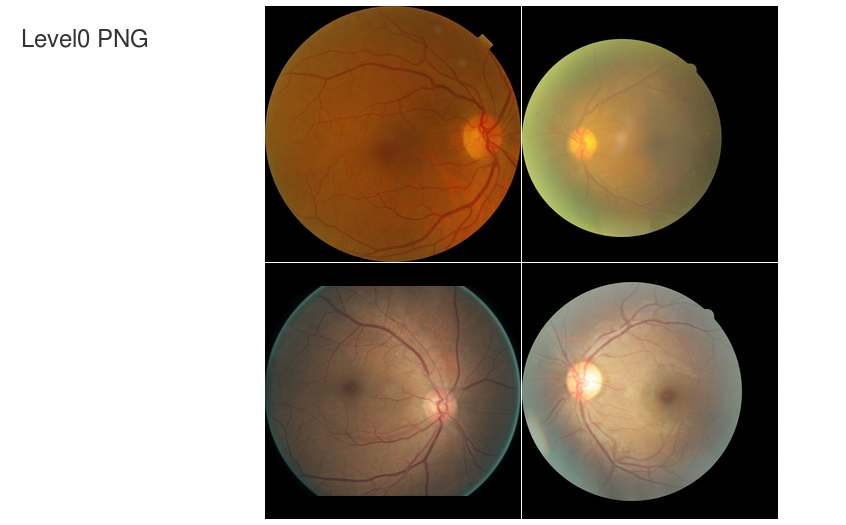
\includegraphics[scale=0.5]{images/Level0_Top4.png}
\caption{Top Four Confidence Diagnosis of Level 0}
\label{DR0}
\end{center}
\end{figure}

\begin{figure}[htbp]
\begin{center}
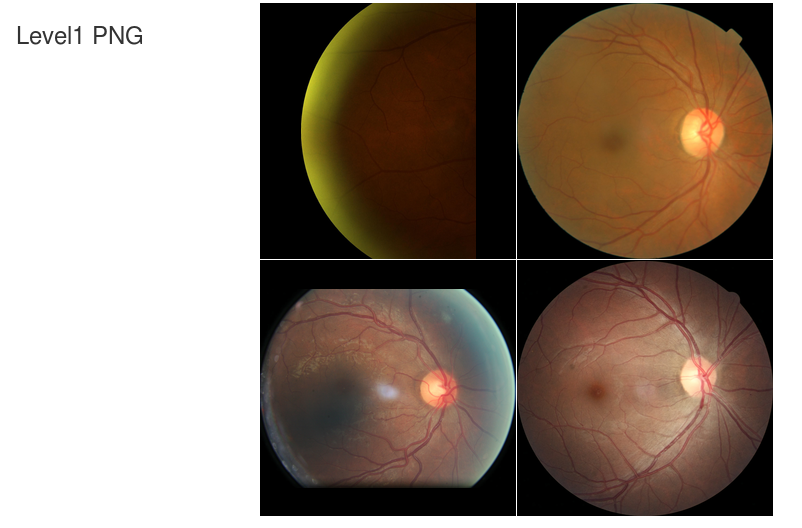
\includegraphics[scale=0.5]{images/Level1_Top4.png}
\caption{Top Four Confidence Diagnosis of Level 1}
\label{DR1}
\end{center}
\end{figure}

\begin{figure}[htbp]
\begin{center}
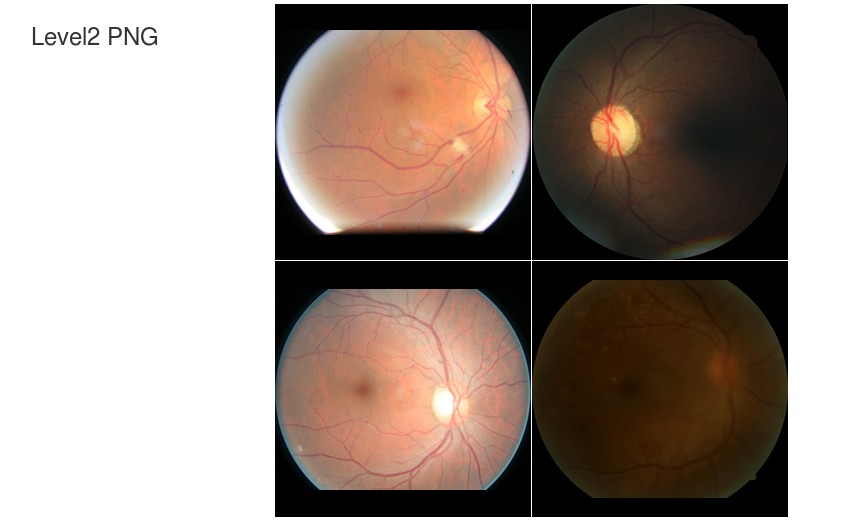
\includegraphics[scale=0.5]{images/Level2_Top4.png}
\caption{Top Four Confidence Diagnosis of Level 2}
\label{DR2}
\end{center}
\end{figure}

\begin{figure}[htbp]
\begin{center}
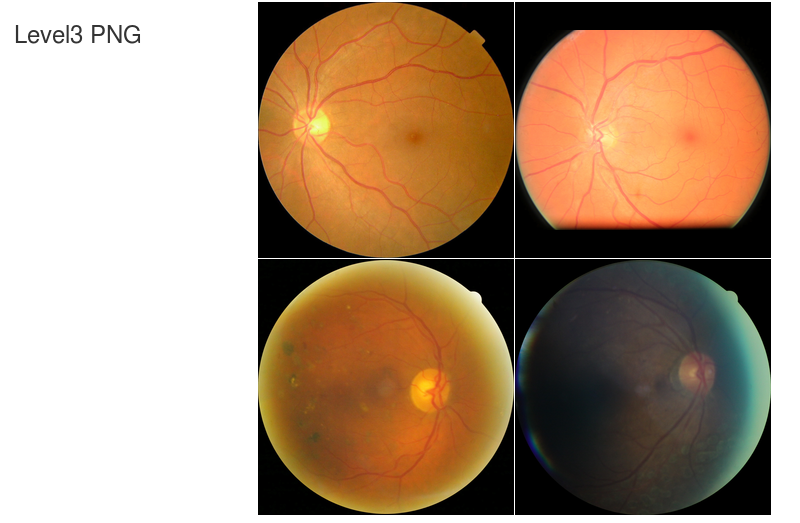
\includegraphics[scale=0.5]{images/Level3_Top4.png}
\caption{Top Four Confidence Diagnosis of Level 3}
\label{DR3}
\end{center}
\end{figure}

\begin{figure}[htbp]
\begin{center}
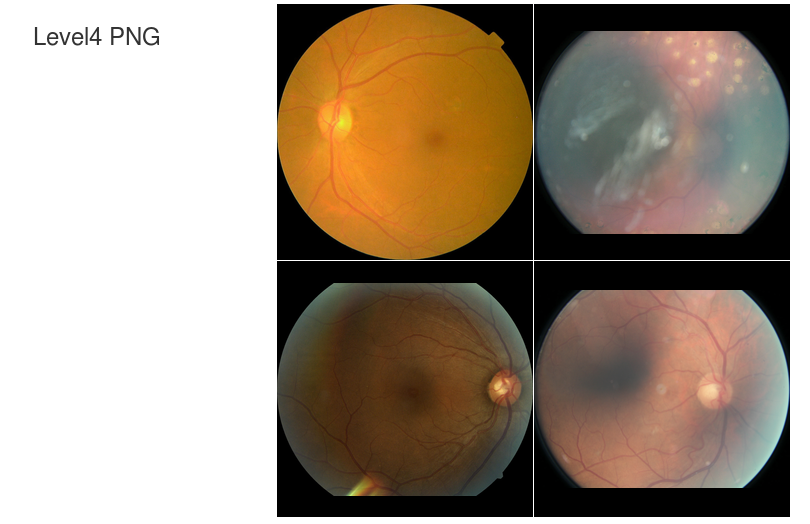
\includegraphics[scale=0.5]{images/Level4_Top4.png}
\caption{Top Four Confidence Diagnosis of Level 4}
\label{DR4}
\end{center}
\end{figure}

\newpage
\section{Conclusion}

This was a very interesting and challenging project. Despite that the final results of the trained network being relatively low compared to the leader board posted on \textit{Kaggle}, (which at the time of this report was $\approx$ 85 $\%$), significant insight was gained into ConvNN implementation and application as a result of the work that went into project.

\newpage
% \nocite{*}
\bibliographystyle{unsrt}
\bibliography{References}


\end{document}